\section{Kết quả thực nghiệm}

\subsection{10 tác vụ}
    \begin{frame}{Dữ liệu thử nghiệm}
        Như trong luận văn
    \end{frame}
    \begin{frame}{Cài đặt thực nghiệm}
        Như trong luận văn
    \end{frame}
    \begin{frame}{Kết quả tối ưu}
        Như trong luận văn
    \end{frame}
    \begin{frame}{Kết quả ghép cặp}
        Như trong luận văn
    \end{frame}

\subsection{50 tác vụ}
    \begin{frame}{Dữ liệu thử nghiệm}
        Như trong luận văn
    \end{frame}
    \begin{frame}{Cài đặt thực nghiệm}
        Như trong luận văn
    \end{frame}
    \begin{frame}{Kết quả tối ưu}
        Như trong luận văn
    \end{frame}
    \begin{frame}{So sánh thời gian chạy}
        Như trong luận văn
    \end{frame}

\subsection{Mujoco tác vụ}
    \begin{frame}{Dữ liệu thử nghiệm}
        Như trong luận văn
    \end{frame}
    \begin{frame}{Cài đặt thực nghiệm}
        Như trong luận văn
    \end{frame}
    \begin{frame}{Kết quả tối ưu}
        Như trong luận văn
    \end{frame}
    \begin{frame}{So sánh thời gian chạy}
        Như trong luận văn
    \end{frame}
    
% \begin{frame}{Experimental setup}
%     \begin{columns}
%         \begin{column}{0.51\linewidth}
%             \begin{exampleblock}{Benchmark}
%             \begin{itemize}
%                 \item 10-task benchmarks, easy to debug, known relationship between tasks
%                 \item 50-task benchmarks, MaTSOO benchmark from the WCCI2020 Competition
%             \end{itemize}
%         \end{exampleblock}
%         \end{column}
%         \begin{column}{0.48\textwidth}
%             \begin{exampleblock}{MFEA/EBSGA/\gls{propose}}
%                 \begin{itemize}
%                     \item Population size: 100
%                     \item rmp: 0.3
%                     \item sbxdi: 2
%                     \item pmdi: 5
%                 \end{itemize}
%             \end{exampleblock}
%         \end{column}
%     \end{columns}
%     \begin{exampleblock}{MaTGA}
%         Use authors' default parameters
%     \end{exampleblock}
% \end{frame}

% \begin{frame}{Result on 10-task benchmark}
%     \begin{table}[H]
%         \begin{tabular}{@{}ccccc@{}}
%             \toprule
%             \textbf{Task} & \gls{propose} & MFEA & MaTGA & EBSGA \\ \midrule
%             $T_1$ & \textbf{3.72E-05}   & 1.31E+00 $(-)$          & 2.45E-04          $(-)$ & 5.58E-04 $(-)$ \\
%             $T_2$ & \textbf{6.48E-06}   & 1.27E+00 $(-)$          & 4.75E-04          $(-)$ & 6.10E-05 $(-)$ \\
%             $T_3$ & \textbf{4.35E-07}   & 1.17E+00 $(-)$          & \textbf{0.00E+00} $(\approx)$ & 2.00E-06 $(-)$ \\
%             $T_4$ & \textbf{7.09E-13}   & 3.37E+00 $(-)$          & 1.00E-06          $(-)$ & 1.60E-05 $(-)$ \\
%             $T_5$ & 1.74E+01            & 8.15E+02 $(-)$          & \textbf{2.16E-02} $(+)$ & 3.29E-02 $(+)$ \\
%             $T_6$ & \textbf{7.03E-04}   & 1.99E+01 $(-)$          & 3.61E-03          $(-)$ & \textbf{8.59E-04} $(\approx)$ \\
%             $T_7$ & 1.00E-02            & 1.05E+01 $(-)$          & \textbf{5.57E-04} $(+)$ & 1.60E-03 $(+)$ \\
%             $T_8$ & 1.89E+02            & 2.34E+03 $(-)$          & \textbf{3.40E-02} $(-)$ & 4.73E-02 $(-)$ \\
%             $T_9$ & \textbf{4.00E-07}   & 4.11E+02 $(-)$          & 4.52E-03          $(-)$ & 4.58E-03 $(-)$ \\
%             $T_{10}$ & 2.74E+01            & \textbf{1.54E+01} $(+)$ & 1.57E+01          $(+)$ & 3.41E+01 $(-)$ \\
%             \bottomrule
%         \end{tabular}
%         \caption{The performance of the GA-based evolution many-tasking algorithms of 10-task benchmark after 30 independent runs. $(-, +, and \approx$ denote the corresponding algorithm is significantly worse, better or similar to \gls{propose} after Wilcoxon signed-rank test at $\alpha=0.05 )$}
%         \label{tab:last10}
%     \end{table}
% \end{frame}

% \begin{frame}{Analyse the KL-UCB}
%     \begin{figure}
%         \centering
%         \begin{subfigure}[b]{0.3\linewidth}
%             \centering
%             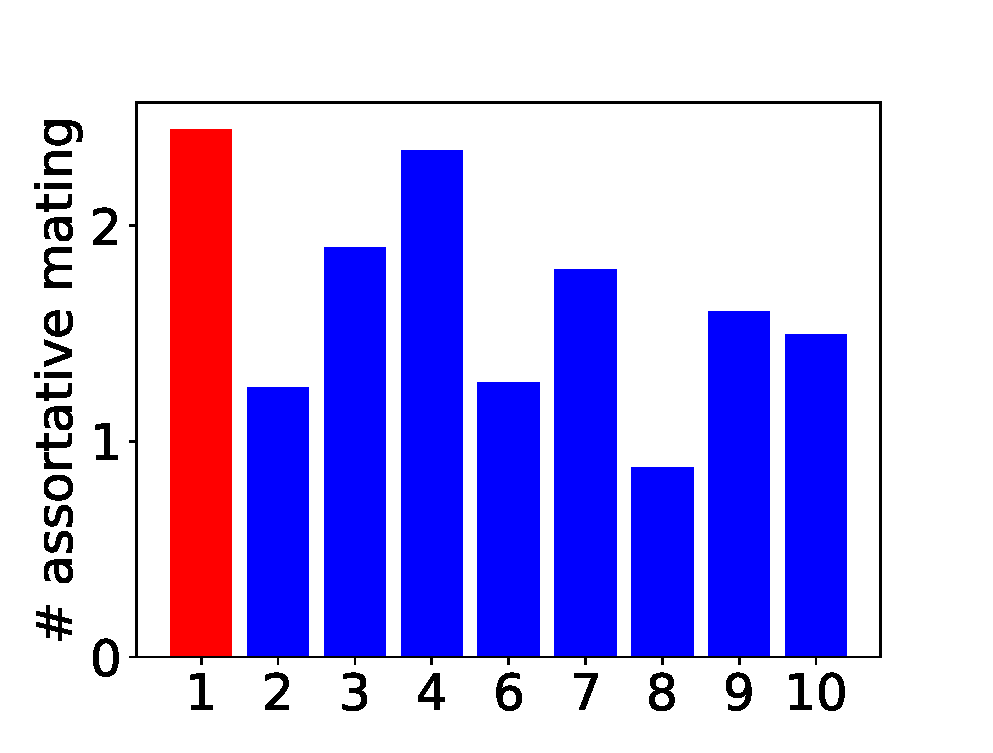
\includegraphics[width=\linewidth]{figure/experiment/bar10/5.eps}
%             \caption{Task 5}
%             \label{fig:bar10-5}
%         \end{subfigure}
%         \hfill
%         \begin{subfigure}[b]{0.3\linewidth}
%             \centering
%             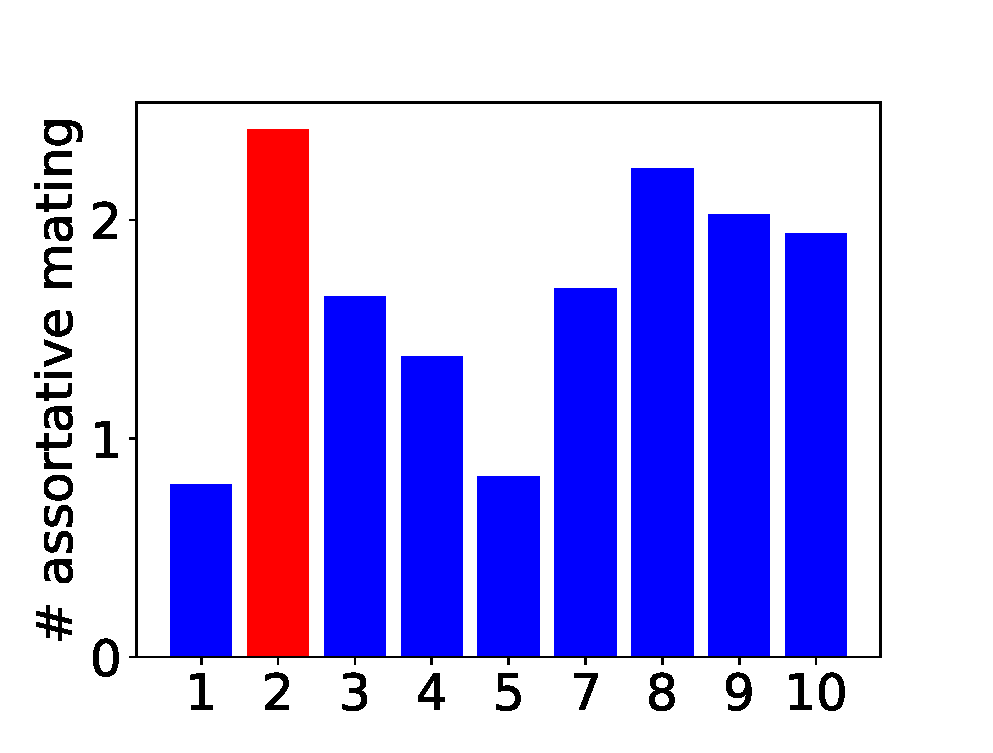
\includegraphics[width=\linewidth]{figure/experiment/bar10/6.eps}
%             \caption{Task 6}
%             \label{fig:bar10-6}
%         \end{subfigure}
%         \hfill
%         \begin{subfigure}[b]{0.3\linewidth}
%             \centering
%             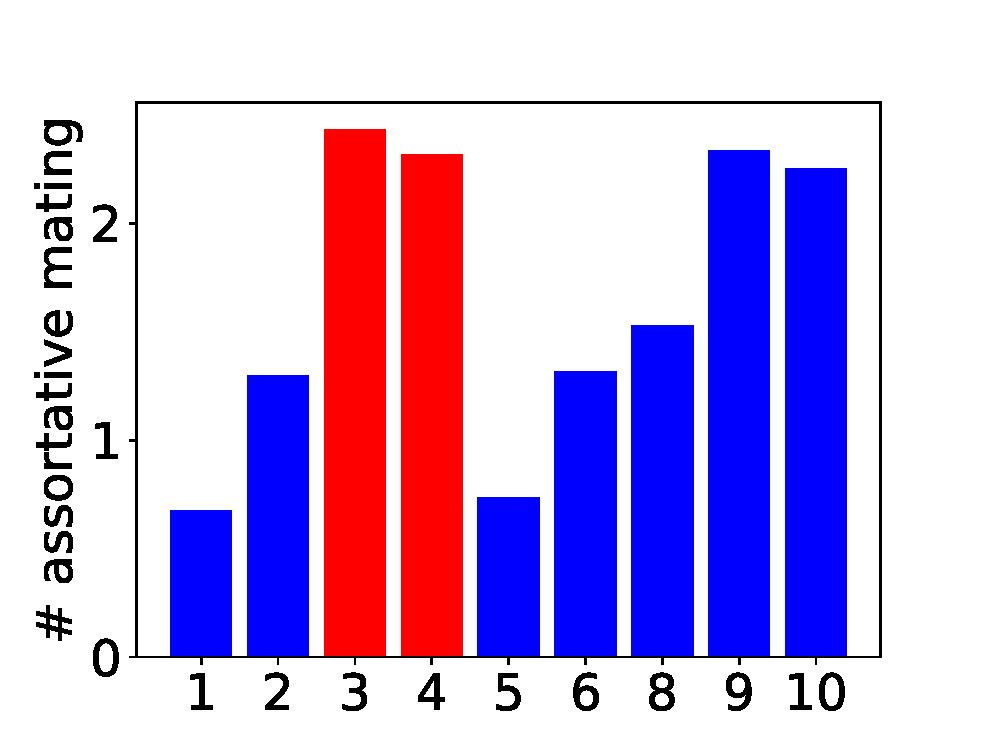
\includegraphics[width=\linewidth]{figure/experiment/bar10/7.eps}
%             \caption{Task 7}
%             \label{fig:bar10-7}
%         \end{subfigure}
%         \hfill
%         \begin{subfigure}[b]{0.3\linewidth}
%             \centering
%             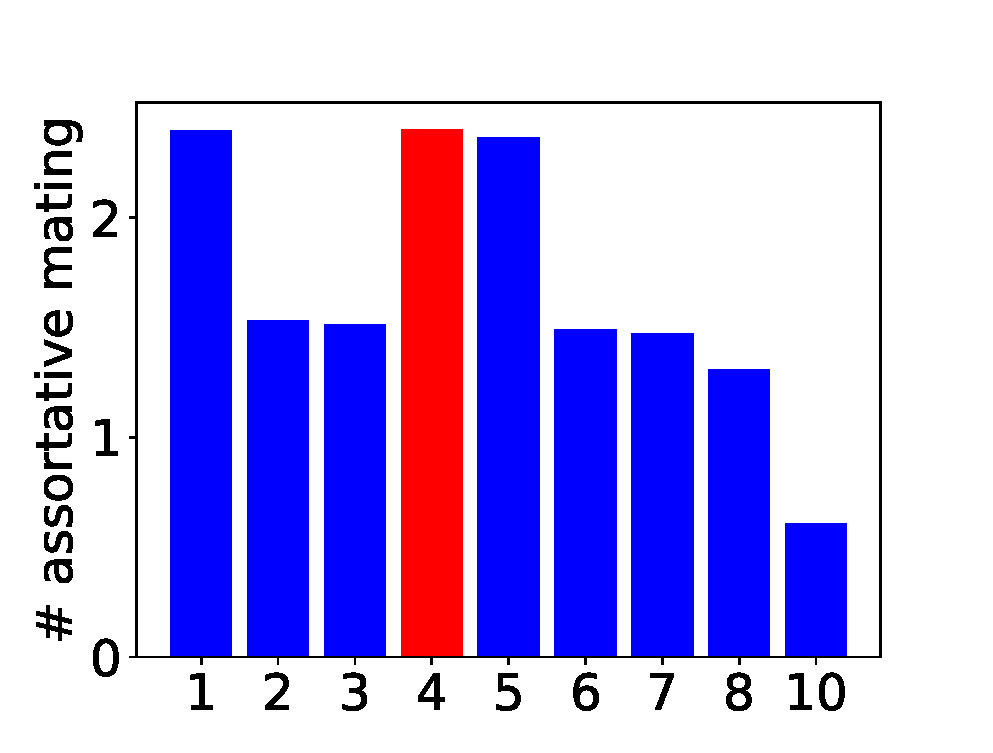
\includegraphics[width=\linewidth]{figure/experiment/bar10/9.eps}
%             \caption{Task 9}
%             \label{fig:bar10-9}
%         \end{subfigure}
%         \hfill
%         \caption{The average times of choosing knowledge transfer target for complex tasks by \gls{propose} with the ideal assisted task is highlighted in red}
%         \label{fig:count10}
%     \end{figure}
% \end{frame}


% \begin{frame}{Result on 50-task benchmark}
%     \begin{table}[hp]
%         \centering
%         \begin{tabular}{@{}ccccc@{}}
%             \toprule
%             \textbf{Benchmark} & \gls{propose} & MFEA & MaTGA & EBSGA \\ \midrule
%             $B_1$    & \textbf{50 (50)} & 0 (0) & 0 (0)           & 0 (0) \\
%             $B_2$    & \textbf{50 (50)} & 0 (0) & 0 (0)           & 0 (0) \\
%             $B_3$    & 8 (0)            & 0 (0) & \textbf{42 (8)} & 0 (0) \\
%             $B_4$    & 17 (9)           & 0 (0) & 0 (0)           & \textbf{33 (33)} \\
%             $B_5$    & \textbf{50 (50)} & 0 (0) & 0 (0)           & 0 (0) \\
%             $B_6$    & \textbf{50 (50)} & 0 (0) & 0 (0)           & 0 (0) \\
%             $B_7$    & 3 (0)            & 0 (0) & 14 (2)          & \textbf{33 (28)} \\
%             $B_8$    & \textbf{30 (28)} & 0 (0) & 0 (0)           & 20 (20) \\
%             $B_9$    & \textbf{42 (42)} & 0 (0) & 0 (0)           & 8 (8) \\
%             $B_{10}$ & 8 (6)            & 2 (0) & 11 (10)         & \textbf{29 (23)} \\
%             \bottomrule
%         \end{tabular}
%         \caption{The performance of the GA-based evolution many-tasking algorithms of 10 benchmarks, each contains 50 tasks, after 30 independent runs. Each entry denotes the number of tasks which the corresponding algorithm is better than other algorithms. The figure within the curly brace indicates the number of tasks which the corresponding algorithm is the best, and it is significantly better than the $2^{nd}$ place algorithm, tested by Wilcoxon signed-rank test at $\alpha=0.05 )$}
%         \label{tab:last50}
%     \end{table}
% \end{frame}

% \begin{frame}{Execution time analysis}
% \begin{figure}[H]
%     \centering
%     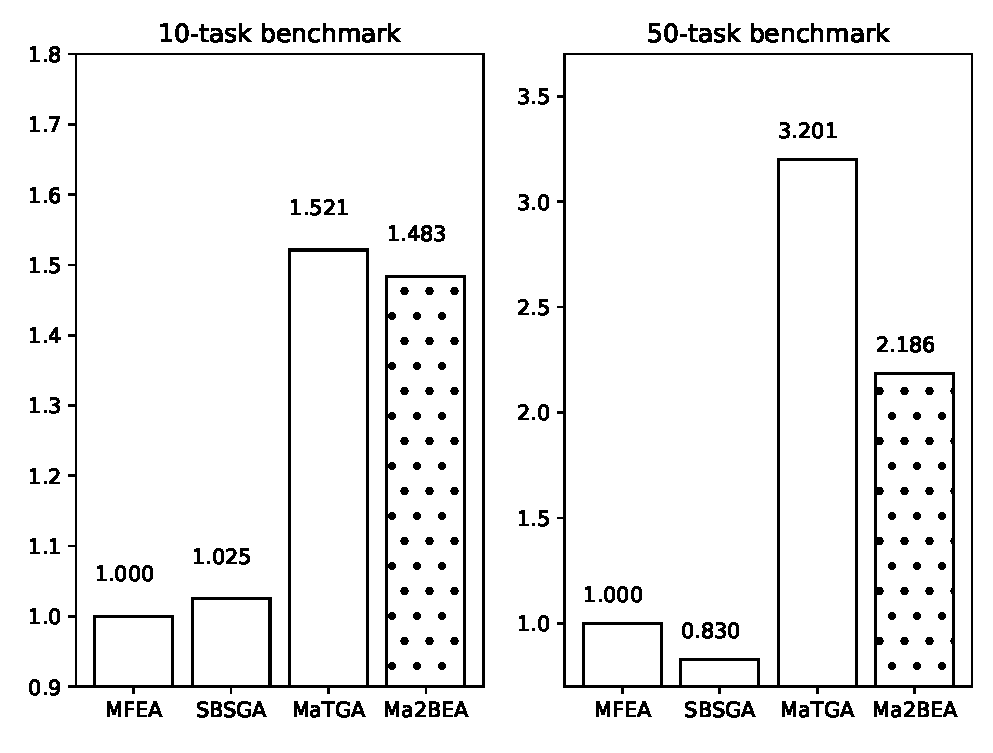
\includegraphics[width=0.7\linewidth]{figure/experiment/runtime.eps}
%     \caption{Execution of different algorithms on two many-tasking benchmarks divided by execution time of MFEA on the same runtime environment}
%     \label{fig:runtime}
% \end{figure}
% \end{frame}